\documentclass[main.tex]{subfiles}
\begin{document}

\section{QED process at the lowest order}

\marginpar{Wednesday\\ 2020-6-17, \\ compiled \\ \today}

We will now study \textbf{tree level} processes in QED: this means that we only consider QED processes which have \emph{no loops}.
This usually corresponds to considering the leading order. 

We will look at three processes explicitly: 
\begin{enumerate}
    \item \(e^{+} e^{-} \to \mu^+ \mu^-\) scattering;
    \item \(e^{-}\) scattering by an external EM field;
    \item \(e^{-} \gamma \to e^{-} \gamma \) (Compton) scattering.
\end{enumerate}

The techniques we will apply here will generalize to any tree-level QED process. 

\subsection{Two-flavoured QED Lagrangian}

In order to consider the \(e^{+} e^{-} \to \mu^+ \mu^-\) process we need a QFT description of the muon as well as the electron: so, we write a Lagrangian with both terms. It reads: 
%
\begin{align}
\mathscr{L}^{(2)}_{\text{QED}} = - \frac{1}{4} F^{\mu \nu } F_{\mu \nu }
- \frac{1}{2 \xi } \qty(\partial_{\mu } A^{\mu })^2
+ \overline{\psi}_{e} \qty(i \slashed{\DD}_e - m_e) \psi_{e}
+ \overline{\psi}_{\mu} \qty(i \slashed{\DD}_\mu - m_\mu) \psi_{\mu}
\,,
\end{align}
%
where the covariant derivative associated with the particle species \(j\) contains the charge of that particle, \(q_j\):
%
\begin{align}
\slashed{\DD}_j = \gamma^{\mu } \qty(\partial_{\mu } + i q_j A_{\mu })
\,.
\end{align}

This holds in general, but in our case \(q_e = q_\mu = -e\). 
The Lagrangian \(\mathscr{L}^{(2)} _{\text{QED}}\) has a \(U(1)\) gauge symmetry, whose action is 
%
\begin{align}
A^{\mu }(x) & \to A^{\mu }(x ) - \partial_{\mu } \alpha (x)  \\
\psi_{e, \mu }(x) & \to e^{iq \alpha (x)} \psi_{e, \mu }(x)
\,;
\end{align}
%
and a \(U(1)_{e} \times U(1)_{\mu }\) global symmetry, whose action is 
%
\begin{align}
A^{\mu }(x) &\to A^{\mu }(x)  \\
\psi_{e, \mu } (x ) & \to e^{i \beta_{{e, \mu }}} \psi_{e, \mu }
\,,
\end{align}
%
where \(\beta_{e, \mu }\) are two (possibly different) constants. 

\subsection{\(e^{+}e^{-} \to f^{+} f^{-}\) unpolarized scattering}

Here, \(e^{\pm}\) are electron and positron, while \(f\) is a generic spin \(1/2\) fermion. 

We make the assumption that the couplings are \textbf{diagonal} in flavour space: this means that there is no term in the Lagrangian which couples \(e\) and \(f\) explicitly, instead they are both coupled to the EM field and interact in that way. 

\todo[inline]{Is this the correct interpretation?}

Then, the QED vertex for this interaction looks like 
%
\begin{align}
\feynmandiagram[baseline=(v.base), horizontal=v to p]{
    f1 [particle = {\(f^{-}\)}] -- [fermion] v [label= left : \(\mu \)],
    f2 [particle = {\(f^{+}\)}] -- [anti fermion] v,
    v -- [photon] p [particle = \(\gamma \)]
};
= - i q_f \gamma^{\mu }
\,.
\end{align}

This holds for the generic fermion \(f\), so for the electron as well. 
So, if \(f \neq e\) we only have one diagram contributing to this interaction, at second order and at tree level: 
\begin{figure}[ht]
\centering
\feynmandiagram[layered layout, extra large, horizontal = ia to ib]{
e1 [particle = {\(e^{-}_{r}\)}] -- [fermion, momentum = \(\vec{p}\)] ia [label = -45: \(-i q_e \gamma_{\mu }\)] -- [photon, momentum = {\(\vec{k}= \vec{p}+\vec{q}\)}] ib [label = 235 : {\(-iq_f \gamma_{\nu }\)}] -- [fermion, momentum = {\(\vec{p}'\)}] e2 [particle = {\(f^{-}_{r'}\)}],
p1 [particle = {\(e^{+}_{s}\)}] -- [anti fermion, momentum' = \(\vec{q}\)] ia,
ib -- [anti fermion, momentum' = \(\vec{q}'\)] p2 [particle = {\(f^{+}_{s'}\)}]
};
\caption{Tree level diagram for electron-fermion interaction.}
\label{fig:electron-fermion-tree-level}
\end{figure}

Also, we denote the mass of the electron as \(m\) and the mass of the other fermion as \(M\).

The whole diagram can just as well be flipped: the incoming and outgoing direction of the momenta is arbitrary. 
Because of momentum conservation, \(\vec{k} = \vec{p} + \vec{q} = \vec{p}' + \vec{q}'\).

The Feynman amplitude is given by the Feynman rules: 
%
\begin{align}
\mathcal{M}_{ef} = (-i q_f) (-i q_e)
\overline{u}_{r'} (p') \gamma_{\nu } v_s' (q')
\overline{v}_{s} (q) \gamma_{\mu} u_r (p)
\widetilde{D}^{\mu \nu } (k)
\,,
\end{align}
%
where the photon propagator in the gauge-fixing Lagrangian is given by 
%
\begin{align}
\widetilde{D}^{\mu \nu } (k) = \frac{-i}{k^2 + i \epsilon }
\qty(\eta^{\mu \nu } - \frac{k^{\mu }k^{\nu }}{k^2} (1 - \xi ))
\overset{\xi =1}{=}
\frac{-i}{k^2 + i \epsilon }
\eta^{\mu \nu }
\,.
\end{align}

Observables do not depend on the choice for \(\xi \), so we can set it to one without worry. 

\todo[inline]{But the EOM for the EM field depend on \(\xi \) explicitly!}

Also, we will now start implying the \(+i \epsilon \) term.

Now, in order to write the Feynman amplitude more explicitly we introduce the Mandelstam variables: 
%
\begin{align}
s &= (p+q)^2 = (p' + q')^2 \\
t &= (p-p')^2 = (q - q')^2 \\
u &= (p-q')^2 = (q - p')^2 
\,,
\end{align}
%
which are a useful covariant scalar description of the kinematics. 
With these conventions, the Feynman amplitude reads: 
%
\begin{align}
\mathcal{M}_{ef} = \frac{i q_e q_f}{s} 
\overline{u}_{r'} (p') \gamma^{\mu } v_s' (q')
\overline{v}_{s} (q) \gamma_{\mu} u_r (p)
\,,
\end{align}
%
since \(k^2 = s\), as \(k = p+q\).
Now the real matrix-crunching starts: we want to find \(\abs{\mathcal{M}}^2 = \mathcal{M} \mathcal{M}^{*}\), which will be needed in the computation of the cross section, so we make it explicit: 
%
\begin{align}
\abs{\mathcal{M}}^2 = \qty(\frac{q_e q_f}{s})^2 
\qty(\overline{u} (p') \gamma^{\mu } v (q')) \qty(\overline{v}(q) \gamma_{\mu } u(p)) 
\qty(\overline{u} (p') \gamma^{\nu } v (q'))^{*} \qty(\overline{v}(q) \gamma_{\nu } u(p))^{*}
\,,
\end{align}
%
which we can manipulate: consider the conjugate bits
%
\begin{align}
\qty(\overline{u} (p') \gamma^{\nu } v (q'))^{*} 
&= u_{\alpha }(p') \qty( \gamma^{0 *} \gamma^{\nu *})_{\alpha \beta } v^{*}_{\beta } (q')  \\
&= v^{*}_{\beta }(q')\qty( \gamma^{0 *} \gamma^{\nu *} \gamma^{0} \gamma^{0})_{\alpha \beta }
u_\alpha (p')    \\
&= v^{*}_{\beta }(q')\qty( \gamma^{\nu \top} \gamma^{0})_{\alpha \beta }
u_\alpha (p')  \\
&= v^{*}_{\beta } (q') (\gamma^{0 \top} \gamma^{\nu })_{\beta \alpha } u_\alpha (p')  \\
&= \overline{v}_{\beta } (q') \gamma^{\nu  } u_\alpha (p')
\,,
\end{align}
%
where we used the identity \eqref{eq:gamma-matrices-identity}, noticing the fact that it can be adapted into 
%
\begin{align}
\gamma^{0} \gamma^{\nu , \top} \gamma^{0} = \gamma^{\nu *}
\,,
\end{align}
%
since \(\gamma^{0} = \gamma^{0 \dag} = \gamma^{0 \top} = \gamma^{0 *}\). The symbol \(\top\) means transpose, so that \(\top * = \dag\). Also, \(\qty(\gamma^{0})^2 = \mathbb{1}\) so a pair of them can be inserted anywhere.

This all means that our Dirac spinor construction is well-behaved under conjugation: \((\overline{u} \gamma v)^{*} = \overline{v} \gamma u\), as it should be. 
This means that we can write the probability as: 
%
\begin{align}
\abs{\mathcal{M}}^2 = \qty(\frac{q_e q_f}{s})^2 
\underbrace{\qty(
\overline{u}_{r'}(p') \gamma^{\mu } v_{s'}(q') \overline{v}_{s'} (q') \gamma^{\nu } u_{r'}(p')
)}_{\text{muon}}
\underbrace{\qty(
\overline{v}_{s}(q) \gamma_{\mu} u_r (p) \overline{u}_{r}(p) \gamma_{\nu } v_s(q)
)}_{\text{electron}}
\,.
\end{align}

We want to consider the \textbf{unpolarized} \(\abs{\mathcal{M}}^2\), so we need to average over the 4 initial polarizations (\(r, s\)), and sum over the final polarizations (\(r', s'\)).
The factor \(4\) is calculated as \((2s_{e^{-}}+1) (2s_{e^{+}}+1)\). 

We make the spinorial indices explicit and find: 
%
\begin{align}
\abs{\mathcal{M}}^2 = 
\qty( \frac{q_e q_f}{2 s})^2 
\underbrace{\sum _{r'} u_{r'}^{ \delta'} \overline{u}^{\alpha '}_{r'}
\sum _{s'} v_{s'}^{ \beta'} \overline{v}^{\gamma '}_{s'}}_{\text{muon, mass }M}
(\gamma^{\mu })_{ \alpha ' \beta '}
(\gamma^{\nu })_{ \gamma ' \delta '}
\underbrace{\sum _{r} u_{r}^{ \delta} \overline{u}^{\alpha }_{r}
\sum _{s} v_{s}^{ \beta} \overline{v}^{\gamma }_{s}
}_{\text{electron, mass }m}
(\gamma_{\mu })_{ \alpha  \beta }
(\gamma_{\nu })_{ \gamma  \delta }
\,.
\end{align}

Now, objects in the form \(\sum _{r} u_r \overline{u}_{r}\) are \textbf{projectors} in spinor space: specifically, they are the ones defined in equation \eqref{eq:energy-projectors-spinor} (without the mass in the denominator). 
So, we can write the ones corresponding to the electron as: 
%
\begin{align}
\sum _{r} u_r (p) \overline{u}_r (p) &= 2 m \Lambda_{+} (p) = \slashed{p} + m \\
\sum _{s} v_s (p) \overline{v}_s (p) &= -2 m \Lambda_{-} (p) = \slashed{p} - m
\,,
\end{align}
%
and similarly for the ones of the other fermion.
So, writing all the terms in order we find: 
%
\begin{align}
\begin{split}
\abs{\mathcal{M}}^2 &= 
\qty( \frac{q_e q_f}{2 s})^2 
(\gamma^{\mu })_{ \alpha ' \beta '}
(\slashed{q}' - M)_{\beta ' \gamma '}
(\gamma^{\nu })_{ \gamma ' \delta '}
\qty(\slashed{p}' + M)_{ \delta ' \alpha '} \\
&\phantom{=}\ 
(\gamma_{\mu })_{ \alpha  \beta }
(\slashed{q} - m)_{\beta  \gamma }
(\gamma_{\nu })_{ \gamma  \delta }
\qty(\slashed{p} + m)_{ \delta  \alpha }
\end{split}  \\
&= 
\qty( \frac{q_e q_f}{2 s})^2 
\Tr [\gamma^{\mu } (\slashed{q}' - M) \gamma^{\nu } (\slashed{p}' + M)]
\Tr [\gamma_{\mu } (\slashed{q} - m) \gamma_{\nu } (\slashed{p} + m)]
\,,
\end{align}
%
so we have the result: summing over the initial and final polarizations corresponds to taking a trace over the fermionic lines. 

This makes sense: there are no free spinorial indices in the probability, so we must trace them all away. 

\todo[inline]{He then makes an example in which we have a fermionic loop which yields a trace, but this was not the case here... How do these connect? Do we need a loop or not?}

This is similar to the Feynman rules: instead of the propagator \(\widetilde{S}(p)\) we plug in the projector \(\Lambda_{\pm }(p)\). 

\begin{claim}
The traces are equal to: 
%
\begin{align} \label{eq:fermion-loop-trace-identity}
\Tr [\gamma_{\mu } (\slashed{q} - m) \gamma_{\nu } (\slashed{p} + m)] &= 
4 \qty[\qty(p_{\mu } p_{\nu } + q_{\mu } p_{\nu }) - (m^2 + p \cdot q) \eta_{\mu \nu}] \\
\Tr [\gamma^{\mu } (\slashed{q}' - M) \gamma^{\nu } (\slashed{p}' + M)] 
&= 4 \qty[\qty(p_{\mu }' p_{\nu }' + q_{\mu }' p_{\nu }') - (M^2 + p' \cdot q') \eta_{\mu \nu}] 
\,.
\end{align}
\end{claim}

\begin{proof}
We do the first one (so we do not have to write many primes), the other one is precisely analogous. 
We make the product explicit, using the linearity of the trace:
%
\begin{align}
\Tr [\gamma_{\mu } (\slashed{q} - m) \gamma_{\nu } (\slashed{p} + m)]
&= \Tr[ \gamma_{\mu } \slashed{q} \gamma_{\nu } \slashed{p}]
-m\Tr[\gamma_{\mu } \gamma_{\nu } \slashed{p}]
+m\Tr[\gamma_{\mu } \slashed{q} \gamma_{\nu }]
-m^2 \Tr[\gamma_{\mu } \gamma_{\nu }]
\,.
\end{align}

Now, we have terms with two, three and four gamma matrices. 

\begin{claim}
The trace of an odd number of gamma matrices vanishes.
\end{claim}

\begin{proof}
Recall the definition of the matrix \(\gamma5 \) \eqref{eq:gamma5-definition}. Its square is the identity: so, we can insert it anywhere. So, let us take: 
%
\begin{align}
\Tr[ \prod_{i=1}^{2n+1} \gamma^{\mu_{i}} ] &= \Tr[\gamma^{5} \gamma^{5}\prod_{i=1}^{2n+1} \gamma^{\mu_{i}}]  \\
&= \Tr[\gamma^{5}\prod_{i=1}^{2n+1} \gamma^{\mu_{i}} \gamma^{5}] \marginnote{Cyclicity of the trace.}  \\
&= (-)^{2n+1} \Tr[\gamma^{5} \gamma^{5}\prod_{i=1}^{2n+1} \gamma^{\mu_{i}} ]  \marginnote{Anticommutation, \(\qty{\gamma^{5}, \gamma^{\mu }} = 0\).}\\
&= (-)^{2n+1} \Tr[\prod_{i=1}^{2n+1} \gamma^{\mu_{i}} ] \marginnote{Cyclicity of the trace.}
\,.
\end{align}

So, the trace is equal to minus itself, so it vanishes. 
\end{proof}

With this, we can throw away the terms with an odd number of \(\gamma\) matrices: so, we are left with 
%
\begin{align}
\Tr [\gamma_{\mu } (\slashed{q} - m) \gamma_{\nu } (\slashed{p} + m)]
&= \Tr[ \gamma_{\mu } \slashed{q} \gamma_{\nu } \slashed{p}]
-m^2 \Tr[\gamma_{\mu } \gamma_{\nu }]
\,,
\end{align}
%
and we can evaluate the two pieces separately. 
For the second, we have 
%
\begin{align}
\Tr[\gamma_{\mu } \gamma_{\nu }] &= \Tr[\qty{\gamma_{\mu }, \gamma_{\nu }}] - \Tr[\gamma_{\nu } \gamma_{\mu }]  \\
&= 2 \eta_{\mu \nu } \Tr[\mathbb{1}]
- \Tr[\gamma_{\mu } \gamma_{\nu }] \marginnote{Cyclicity of the trace.}  \\
2 \Tr[\gamma_{\mu }\gamma_{\nu }] &= 2 \eta_{\mu \nu } \times 4 \\
\Tr[\gamma_{\mu }\gamma_{\nu }] &= 4 \eta_{\mu \nu } 
\,.
\end{align}

For the first, instead, we use the following:
\begin{claim}[Unproven]
\begin{align}
\Tr[\gamma_{\mu } \gamma_{\nu }\gamma_{\rho } \gamma_{\sigma }]
= 4 \qty(\eta_{\mu \nu } \eta_{\rho \sigma }
+ \eta_{\mu \sigma } \eta_{\nu \rho }
- \eta_{\mu \rho }\eta_{\nu \sigma })   
\,.
\end{align}
\end{claim}

Combining these, we get: 
%
\begin{align}
\Tr[ \gamma_{\mu } \slashed{q} \gamma_{\rho } \slashed{p}]
-m^2 \Tr[\gamma_{\mu } \gamma_{\rho }]
&= q^{\nu }p^{\sigma } \Tr[\gamma_{\mu } \gamma_{\nu }\gamma_{\rho } \gamma_{\sigma }]
- m^2 \Tr[\gamma_{\mu } \gamma_{\rho }]  \\
&= 4 q^{\nu }p^{\sigma } 
\qty(\eta_{\mu \nu } \eta_{\rho \sigma }
+ \eta_{\mu \sigma } \eta_{\nu \rho }
- \eta_{\mu \rho }\eta_{\nu \sigma })
- 4 m^2 \eta_{\mu \rho }  \\
&= 4 \qty(q_{\mu } p_{\rho } + p_{\mu }q_{\rho } - \eta_{\mu \rho } \qty( p \cdot q + m^2) )
\,.
\end{align}
\end{proof}

The masses are \(p^2 = q^2 = m^2\) and \(p^{\prime 2} = q^{\prime 2} = M^2\); in certain cases (like in electron-muon decay) we can assume that since \(M \gg m\) the mass \(m\) is negligible: \(m \approx 0\). 

With this simplification, several terms cancel and we find: 
%
\begin{align}
\abs{\mathcal{M}}^2 \approx \qty(\frac{8 q_e^2 q_{\mu}^2}{s^2})
\qty[(p \cdot p') (q \cdot q') + (p \cdot q')(q \cdot p') + M^2 (p \cdot q)]
\,.
\end{align}

\begin{claim}
If, instead, we do not want to neglect \(m\) we find: 
%
\begin{align}
\abs{\mathcal{M}}^2 = \qty(\frac{8 q_e^2 q_{\mu}^2}{s^2})
\qty[(p \cdot p') (q \cdot q') + (p \cdot q')(q \cdot p') + M^2 (p \cdot q) 
+ m^2 (p' \cdot q') + 2 m^2M^2]
\,.
\end{align}
\end{claim}

\begin{proof}
\todo[inline]{To do.}
\end{proof}

Everything we have derived so far is Lorentz-invariant, and the probability is a Lorentz scalar. 
However, we can specify these results to a specific frame in order to make them more concretely useful. 
We choose the center of mass frame. 

\subsubsection{COM frame}

In this frame, the momenta of the electron and positron will look like: 
%
\begin{align}
p = (\omega, \vec{p}) 
\qquad \text{and} \qquad
q = (\omega, -\vec{p})
\,,
\end{align}
%
while the ones of the other two fermions will be 
%
\begin{align}
p' = (\omega, \vec{p}') 
\qquad \text{and} \qquad
q' = (\omega, -\vec{p}')
\,.
\end{align}

The Mandelstam variable \(s\) is equal to \(4 \omega^2\). 
Notice that the energies are equal even though the mass of the incoming particles, \(m\), is possibly different from the one of the outgoing ones, \(M\).  

Let us write out the scalar products between the momenta explicitly: 
%
\begin{align}
p \cdot p' &= \omega^2 - \abs{\vec{p}} \abs{\vec{p}}' \cos \theta \overset{m \approx 0}{\approx} \omega ( \omega - \abs{\vec{p}}' \cos \theta ) \\
p \cdot q' &= \omega^2 + \abs{\vec{p}} \abs{\vec{p}}' \cos \theta \overset{m \approx 0}{\approx} \omega ( \omega + \abs{\vec{p}}' \cos \theta )  \\
p \cdot q &= \omega^2 + \abs{\vec{p}}^2 \overset{m \approx 0}{\approx}
2\omega^2 \marginnote{Used \(\abs{\vec{p}} \approx \omega \).} \\
p' \cdot q' &= \omega^2 + \abs{\vec{p}'}^2 = 2 \omega^2 - M^2 
\marginnote{Used \(\abs{\vec{p}'}^2 = \omega^2-M^2\).}
\,.
\end{align}

This tells us that the primed-frame momentum is given by 
%
\begin{align}
\abs{\vec{p}'}^2 = \omega^2 \qty(1 - \frac{M^2}{\omega^2})
\,.
\end{align}
%
\todo[inline]{The last one is exact! He writes that it is approximated\dots}

Substituting these in, in the \(m \approx 0 \) approximation we find: 
%
\begin{align}
\abs{\mathcal{M}}^2_{CM} &\approx \frac{8 q_e^2 q_f^2}{s^2}
\qty[
2 \omega^{4} 
+ 2 \omega^2 \abs{\vec{p}'}^2 \cos^2\theta + 2 M^2\omega^2
] \\
&\approx e^{4} \qty[
\qty(1 + \frac{M^2}{s}) +   \qty(1 - \frac{4M^2}{s}) \cos^2\theta 
]
\,.
\end{align}

We can substitute this into the expression we know for the differential cross section \eqref{eq:zero-initial-mass-cross-section}: we find 
%
\begin{align}
\dv{\sigma }{\Omega_1 }
&\approx
\frac{1}{64 \pi^2}
\frac{\abs{\vec{p}'}}{\abs{\vec{p}}}
\abs{\mathcal{M}}^2_{CM}  \\
&= \frac{\alpha^2}{4 s} \sqrt{1 - \frac{4M^2}{s}}
\qty[ \qty(1 + \frac{M^2}{s}) +   \qty(1 - \frac{4M^2}{s}) \cos^2\theta ]
\,,
\end{align}
%
where we have introduced \(\alpha_{EM} = e^2 / 4 \pi^2\). 

\begin{enumerate}
    \item This expression is well-defined as long as \(\sqrt{s} > 2M\), which reminds us that if this is not the case the process is kinematically not allowed. 
    \item The \(\cos^2\theta \) term means we have a maximum at the poles \(\theta = 0, \pi \) (that is, the directions from which the electrons were coming) and a minimum at the equator, \(\theta = \pi /2\). This is similar to other vector-fermion interactions. 
    \item Angular momentum is conserved: two spin \(1/2\) particles become one spin-1 one. 
    \item In the ultrarelativistic limit \(\sqrt{s} \gg M, m\) we have 
    %
    \begin{align}
    \dv{\sigma }{\Omega_1 } \approx \frac{\alpha^2}{4 s} \qty(1 + \cos^2 \theta )
    \qquad \text{and} \qquad
    \sigma = \frac{4 \pi }{3} \frac{\alpha^2}{s} 
    \,.
    \end{align}
\end{enumerate}

\subsubsection{Angular momentum conservation}

In order to get angular momentum conservation we need to calculate the polarized cross sections --- those in which we do not average over the polarizations, but instead keep them fixed.

The ones in which angular momentum would not be conserved vanish. The ones which are nonzero in the \emph{ultrarelativistic limit} are
%
\begin{align}
\abs{\mathcal{M}(-+, - + )}^2 &= \abs{\mathcal{M}_{LL}}^2 = 
e^{4} \qty(1 + \cos \theta )^2 \\
\abs{\mathcal{M}(+ -, + -)}^2 &= \abs{\mathcal{M}_{RR}}^2 = 
e^{4} \qty(1 + \cos \theta )^2 \\
\abs{\mathcal{M}(-+, + -)}^2 &= \abs{\mathcal{M}_{LR}}^2 = 
e^{4} \qty(1 - \cos \theta )^2 \\
\abs{\mathcal{M}(+ -, - + )}^2 &= \abs{\mathcal{M}_{RL}}^2 = 
e^{4} \qty(1 - \cos \theta )^2 
\,,
\end{align}
%
where the four signs denote the spins of the incoming and outgoing particles.

\begin{figure}[ht]
\centering
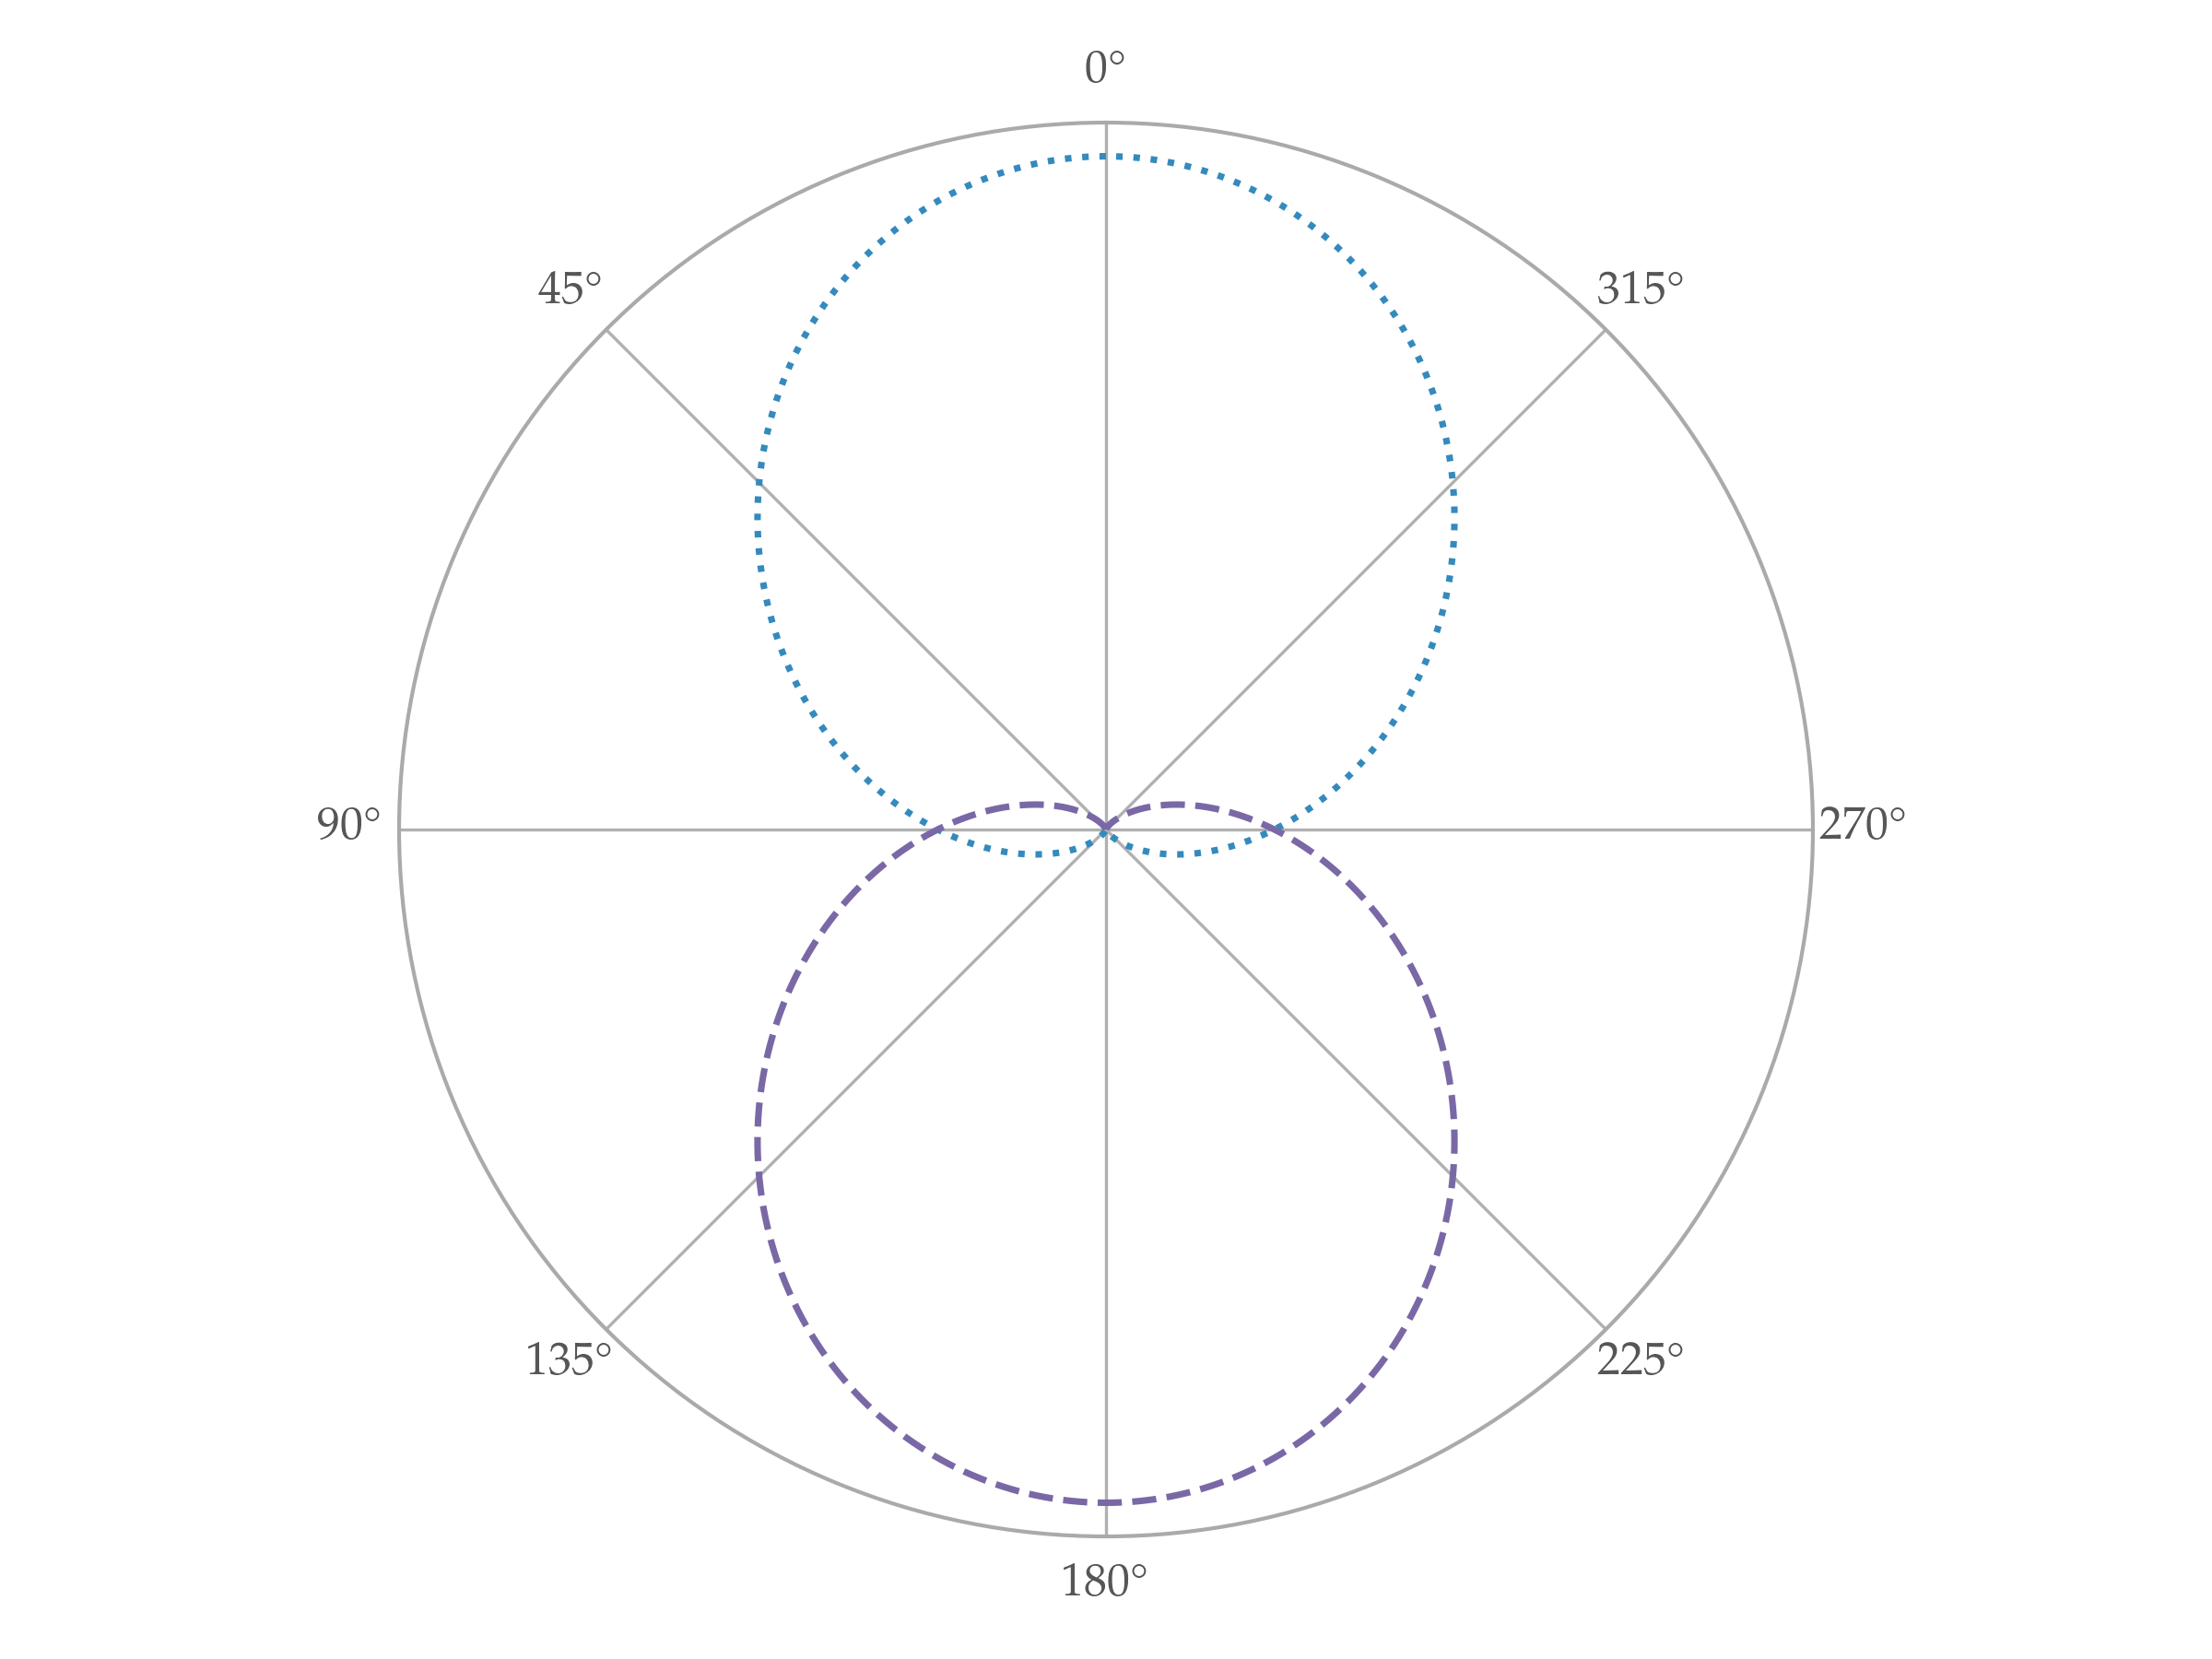
\includegraphics[width=\textwidth]{figures/angular_distribution.png}
\caption{Angular distribution: the dotted line is \(LL\) or \(RR \), the dashed line is \(LR\) or \(RL\). }
\label{fig:angular_distribution}
\end{figure}

We can see in figure \ref{fig:angular_distribution} that in all the cases \(\theta = 0\) and \(\theta = \pi \) correspond to either zero or the maximum probability. 
For the spin-preserving interactions, we have that \(\theta = \pi \) is forbidden, for the spin-flipping ones \(\theta = 0\) is. 

In order to understand this, let us consider the first of the two: we have two incoming electrons with opposite helicities, so their spins will be aligned. 
If, say, we measure spin with respect to the \(z\) axis which is aligned with \(e^{-}\)'s trajectory, we will have \(s_z = -1/2 - (+ 1/2) = -1\) for the total initial spin if the initial spin configuration is \(+ -\).

If the final spin configuration is \(- +\) and the angle is \(\pi \), that means that the fermion \(f^{-}\) with helicity \(-\) is going along positive \(z\), and the fermion \(f^{+}\) with helicity \(+\) is going along negative \(z\), so the total spin will be \(s_z = +1\). 

\todo[inline]{Hold on, something is not super clear: are these quantum numbers actually helicities?}

The unpolarized probability is found by adding all of the \(\abs{\mathcal{M}}^2\) together. 

\begin{claim}
The unpolarized cross sections for the processes \(e^{-} f \to e^{-} f\) and \(e^{-} \overline{f} \to e^{-} \overline{f}\) in the ultrarelativistic limit are respectively: 
%
\begin{align}
\dv{\sigma }{\Omega_1 }
&= \frac{\alpha^2}{4 t} \qty(1 + \cos^2 \theta ) \\
\dv{\sigma }{\Omega_1 }
&= \frac{\alpha^2}{4 u} \qty(1 + \cos^2 \theta )
\,.
\end{align}
\end{claim}

\begin{proof}
The Feynman diagram is the same (rotated by \(\pi /2\) if we follow the conventions), only the kinematics change. 
So, the momentum conservation equation which was 
%
\begin{align}
p + q = p' + q'
\,,
\end{align}
%
now should be written as 
%
\begin{align}
p - p' = q' - q 
\qquad \text{or} \qquad
p - q' = p' - q
\,,
\end{align}
%
where either \(-p'\) or \(-q'\) is the ``new second incoming momentum''. This is equivalent to switching to the other Mandelstam variables.
\end{proof}

\subsection{\(e^{-}f^{-} \to e^{-}f^{-}\) and crossing symmetries}

\begin{figure}[ht]
\centering
\feynmandiagram[vertical = x to y]{
    e1 [particle = {\(e^{-}\)}] -- [fermion] x -- [fermion] e2 [particle = {\(e^{-}\)}],
    x -- [photon, momentum = {\(k = p-p' = q-q'\)}] y ,
    f1 [particle = {\(f^{-}\)}] -- [anti fermion] y -- [anti fermion] f2 [particle = {\(f^{-}\)}]  
};
\caption{Diagram for \(e^{-}f^{-} \to e^{-}f^{-}\).}
\label{fig:efef-feynman-diagram}
\end{figure}

The Feynman diagram for this interaction is shown in figure \ref{fig:efef-feynman-diagram}. The square of the modulus of \(k\) is the Mandelstam variable \(t = k^2 = (p - p')^2\). 
Because of this, this is called the \(t\)-channel. 

The corresponding Feynman amplitude (with \(\xi = 1\)) is 
%
\begin{align}
\mathcal{M} = i \frac{q_e q_f}{t} 
\qty(\overline{u}_{s'} (p') \gamma^{\mu } u_s (p))
\qty(\overline{u}_{r'} (q') \gamma^{\mu } u_r (q))
\,.
\end{align}

Notice that this has a pole (a divergence) for \(t = 0\): this is similar to what we had before, but then the pole was in \(s = 0\), which was fine since that would have meant zero center-of-mass energy. 

In everything but that term the amplitude is the same as last section's. The square of the modulus of the unpolarized amplitude is 
%
\begin{align}
\abs{\mathcal{\overline{M}}}^2_{ef} 
=\frac{q_e^2 q_f^2}{t^2} 
\Tr [\qty(\slashed{p} + m) \gamma^{\nu } \qty(\slashed{p}' + m) \gamma^{\mu }] 
\Tr [\qty(\slashed{q} + M) \gamma_{\nu } \qty(\slashed{q}' + m) \gamma_{\mu }] 
\,.
\end{align}

This can be written starting from the \(ee \to ff\) amplitude with the following maps: 
%
\begin{align}
p \to p 
&&
q \to -p'
&&
q' \to -q 
&&
p' \to -q'
\,,
\end{align}
%
which correspond to the cyclic change of Mandelstam variables: \(s, t, u \to t, u, s\). 

Making these substitutions in the final probability yields, in the ultrarelativistic approximation:
%
\begin{align}
\abs{\mathcal{\overline{M}}}^2_{ee} &= 2 e^{4} \qty(\frac{t^2+ u^2}{s^2}) \\
\abs{\mathcal{\overline{M}}}^2_{ff} &= 2 e^{4} \qty(\frac{u^2+ s^2}{t^2})
\,,
\end{align}
%
since we have the ultrarelativistic relations 
%
\begin{align}
s &= 2 p \cdot q = 2 p' \cdot q'  &
t &= -2 p \cdot p' = -2 q \cdot q' & 
u &= -2 p \cdot q' = -2 q \cdot p' 
\,.
\end{align}

These can all be derived from the definitions, assuming \(0=p^2= q^2=\dots\)

In the center of mass frame we have 
%
\begin{align}
\abs{\mathcal{\overline{M}}}^2_{CM} (ef \to ef) &= 2 e^{4} \qty[\frac{4 + (1 + \cos \theta )^2}{(1 - \cos \theta )^2}]  \\
\dv{\sigma }{\Omega_1 }_{CM}(ef \to ef) &= \frac{\alpha^2}{2s}
\qty[\frac{4 + (1 + \cos \theta )^2}{(1 - \cos \theta )^2}]
\,,
\end{align}
%
where \(\theta \) is the angle between the incoming and outgoing electrons. This diverges for \(\theta \to 0\)! 

The relation between the \(e e \to f f \) process and the \(ef \to ef\) process is known as a \textbf{crossing symmetry}. It can be generalized to any process with this structure.

\begin{claim}
If we have a process in which a particle \(\varphi \) appears in the initial state with a momentum \(\vec{p}\), its \(S\)-matrix is equivalent to the matrix of a process in which \(\varphi \)'s antiparticle appears in the final state with its momentum reversed: 
%
\begin{align}
\mathcal{M} (\varphi (\vec{p}) \dots \to \dots)
= \pm \mathcal{M} (\dots \to \overline{\varphi}(-\vec{p}) \dots)
\,.
\end{align}
\end{claim}

Under certain conditions (unspecified here) when considering fermionic lines the minus sign can appear. 

\todo[inline]{Exercise: derive cross section of \(e^{-} f^{+} \to e^{-}f^{+}\).}

\subsection{Scattering by an external EM field}

We have seen how to quantize the electromagnetic field; often though we do not care to analyze its quantum nature, but instead we want to approximate an external EM field as classical. 

\subsubsection{\(e^{-} p \to e^{-} p\) scattering}

Let us consider the process of scattering \(e^{-} p \to e^{-} p\). We choose to work at such energies that the internal structure of the proton does not affect the process, and we just model the proton as a spin \(1/2\) fermion. So, our Lagrangian will be 
%
\begin{align}
\mathscr{L}_{D} &= 
\overline{\psi}_{e} \qty(i \slashed{\partial} -m_e ) \psi_{e} +
\overline{\psi}_{p} \qty(i \slashed{\partial} -M_p ) \psi_{p} +
\mathscr{L} _{\text{int}} \\
\mathscr{L} _{\text{int}} &= \qty(q_e \overline{\psi}_{e} \gamma^{\mu } \psi_{e} + q_p \overline{\psi}_{p} \gamma^{\mu }\psi_{p}) A_{\mu }
\,.
\end{align}

The lowest order of the scattering is given by the second-order matrix element 
%
\begin{align}
S_{(2)} = (-i q_e)(-i q_p) \int \dd[4]{x} \dd[4]{y}
N \qty[ \qty(\overline{\psi} \slashed{A} \psi )_{x}^{e} \qty(\overline{\psi} \slashed{A} \psi )_{y}^{p}]
\,,
\end{align}
%
which can be represented by the usual \(t\)-channel diagram, just like that which is shown in figure \ref{fig:efef-feynman-diagram}. 
The four-momentum of the photon is \(k\), and its square is the Mandelstam variable \(t\). 

The difference from the last section is that then we studied it in the center-of-mass frame, while we want to consider this one in the \textbf{laboratory} frame (in which the proton is at rest) and assuming \(\omega_{e} \ll M\): the collision is at an energy much smaller than a \SI{}{GeV}.

\begin{claim}
The initial momentum of the proton is then \(p_p = (M, \vec{0})\) and its final one is approximately \(p_p' \approx (M, \vec{p}_p') \approx (M, \vec{0})\).
\end{claim}

% This may be non-obvious intuitively: it is a result from kinematics that momentum after the collision is distributed inversely proportionally to the masses of the particles. 

% \todo[inline]{Is the correction to the momentum of the proton also small \emph{compared to the electron's momentum}? This seems relevant.}

This implies that the collision for the electron is approximately elastic: it ``bounces against a wall'', 

\begin{proof}
This is because the energy conservation equation can be written as 
%
\begin{align}
\omega_{e} + M &= \omega'_e  +M + \frac{\abs{p_p'}^2}{2M}  + \order{\frac{\abs{p_p'}^2}{M^2}} \\
\omega_{e} &= \omega'_e + \order{\frac{\abs{p_p'}}{M}}
\,,
\end{align}
%
so we can approximate \(\omega_{e} = \omega_{e}'\), which implies that the scattering is elastic. This also gives us \(\abs{p_e} = \abs{p_e'}\); however the direction of the momentum is not determined. 
\end{proof}

The Mandelstam variable \(t\) is given by: 
%
\begin{align}
t &= (p_e - p_e')^2 = 2 m_e^2 - 2 p_e \cdot p_e' = 2 m_e^2 - 2 \omega_{e}^2 + 2 \vec{p}_e \cdot \vec{p}_e ' \\
&\approx 2 \abs{p_e}^2 \qty(\cos \theta - 1)  \\
t &= (p_e - p_p')^2 = 2 M^2 - 2 M \omega_{p}' = - \abs{\vec{p}_p'}^2
\,,
\end{align}
%
so we have the following approximate expression for the scattering angle: 
%
\begin{align}
\cos \theta \approx 1 - \frac{1}{2} \frac{\abs{\vec{p}_p'}^2}{\abs{p_e}^2}
\,.
\end{align}

Now we can take two approaches: either we calculate the cross section imposing the laboratory-frame kinematics and the elastic-scattering approximation; or we consider the classical particle as the source of an external electromagnetic field. 

\subsubsection{Lab-frame quantum calculation}

With the \(\xi = 1 \) gauge fixing for the EM field, the Feynman amplitude reads: 
%
\begin{align}
\mathcal{M} = i \frac{q_e q_p}{k^2} 
\qty(\overline{u}_{r'} (p'_e) \gamma^{\mu } u_r (p_e))
\qty(\overline{u}_{s'} (p'_p) \gamma_{\mu } u_s (p_p))
\,,
\end{align}
%
and with our approximations the proton current reads: 
%
\begin{align}
\overline{u}_{s'} (p'_p) \gamma_{\mu } u_s (p_p)
= 2 M \left[\begin{array}{cc}
\xi ^{\top}_{s'} & 0
\end{array}\right]
\gamma^{\mu } 
\left[\begin{array}{c}
\xi_{s} \\ 
0
\end{array}\right]
= 2 M \delta_{s s'}
\eta^{\mu 0}
\,,
\end{align}
%
since only \(\gamma^{0}\) has nonvanishing entries in the upper left \(2 \times 2\) block. 
Therefore, we have 
%
\begin{align}
\mathcal{M} = i \frac{q_e q_p}{k^2} 
\qty(\overline{u}_{r'} (p'_e) \gamma^{0 } u_r (p_e))
2M \delta_{s s'}
\,,
\end{align}
%
so we can calculate the unpolarized amplitude as usual: 
%
\begin{align}
\abs{\mathcal{\overline{M}}}^2
&= \qty(\frac{q_e q_p}{k^2})^2
\qty( \frac{1}{2} \sum _{s s'}) \qty( \frac{1}{2} \sum _{rr'})
4M^2 \delta_{s s'}
\overline{u}_{r'} (p'_e) \gamma^{0} u_r (p_e) 
\overline{u}_{r} (p_e) \gamma^{0} u_{r'} (p_e')  \\
&= \qty(\frac{q_e q_p}{k^2})^2
2 M^2 \Tr[(\slashed{p}_e + m_e) \gamma^{0} (\slashed{p}' + m_e)\gamma^{0}]
\marginnote{\(\sum _{ss'} \delta_{ss'} = 2\).}  \\
% &= \qty(\frac{q_e q_p}{k^2})^2
% 2 M^2 
% \Tr[(\slashed{p}_e + m_e) \gamma^{0} (\slashed{p}' + m_e)\gamma^{0}]  \\
&= \qty(\frac{q_e q_p}{k^2})^2
2 M^2
\times 4
\qty(2 p_e^{0} p_e^{\prime 0} - (- m_e^2 + p_e \cdot p_e^{\prime })\eta_{00}) \marginnote{Used \eqref{eq:fermion-loop-trace-identity}, adapting the sign of the \(m^2\) term: here it is plus.}  \\
&= \qty(\frac{q_e q_p}{k^2})^2
2 M^2
\times 4
\qty(2 \omega_{e}^2 - (- m_e^2 + \omega_{e}^2- \abs{p_e}^2 \cos \theta ) )  \\
&= \qty(\frac{q_e q_p}{k^2})^2
2 M^2
\times 4  \qty(\omega_{e}^2 + m_e^2 + \abs{p_e}^2 \cos \theta )  \\
&= 8 \qty(\frac{q_e q_p}{k^2})^2
M^2 \qty(2 \omega_{e}^2 - \abs{p_e}^2 + \abs{p_e}^2 \cos \theta )  \\
&= 16 \qty(\frac{q_e q_p}{k^2})^2
\frac{M^2}{\omega_{e}^2} \qty(1 - \frac{\abs{p_e}^2}{2 \omega_{e}^2} \qty(1 - \cos \theta ))  \\
&= 16 \qty(\frac{q_e q_p}{k^2})^2
M^2 \omega_{e}^2 \qty(1 - v_e^2 \sin^2 \theta / 2)  \\
&= (q_e q_p)^2 \frac{\omega_{e}^2 M^2}{\abs{p_e}^4}
\frac{(1 - v_e^2 \sin^2\theta /2)}{\sin^{4} \theta / 2}
\,,
\end{align}
%
where we used the facts that \(v_e = \abs{p_e} / \omega_{e}\), and 
%
\begin{align}
t &= k^2 = \qty(p_e - p_e')^2 = 2 m_e^2 - 2 \omega_{e}^2 + 2 \abs{\vec{p}_e}^2 \cos \theta  \\
&= -2 \abs{\vec{p}_e} \qty(1 - \cos \theta )  \\
&= -4 \omega_{e}^2 v_e^2 \sin^2 \theta / 2
\,.
\end{align}

Also, we employed the trigonometric identity \(1- \cos \theta = 2 \sin^2 \theta / 2\). 

Then, in the laboratory frame the differential cross section reads 
%
\begin{align}
\dv{\sigma }{\Omega_1 } = \frac{\alpha^2}{4}
\frac{1}{\omega_{e}^2 v_e^2} 
\frac{(1 - v_e^2 \sin^2\theta /2)}{\sin^{4} \theta / 2}
\,.
\end{align}

This describes the scattering of an electron \(e^{-}\) from the potential generated by a proton. In the nonrelativistic limit \(\omega_{e} \approx m_e\), considering a potentially larger nucleus with \(Z\) protons, we have the Rutherford formula: 
%
\begin{align}
\dv{\sigma }{\Omega_1} = \frac{\alpha^2Z^2}{4 m^2 v_e^{4}}
\frac{1}{\sin^{4} (\theta /2)}
\,.
\end{align}

\subsubsection{External EM field approach}

We take the second-order \(S\)-matrix defined before and bracket it with the initial and final states, which both describe an electron with arbitrary momentum and a stationary proton. This yields: 
%
\begin{align}
\begin{split}
S_{fi} &= - q_e \int \dd[4]{x}
\bra{e^{-}_{s} (p'_e)} 
(\overline{\psi}_{e} \gamma^{\mu} \psi_{e})_x 
\ket{e^{-}_{s}(p_e)} \times\\
&\phantom{=}\ \times
\underbrace{\int \dd[4]{y} D^{F}_{\mu \nu } (x-y) 
\bra{p_{r'} (M)} q_p  
(\overline{\psi}_{p} \gamma^{\nu} \psi_{p})_y 
\ket{p_r (M)}}_{\text{proton term}}
\end{split}
\,,
\end{align}
%
and we can rewrite the proton term as 
%
\begin{align}
\int \dd[4]{y} D^{F}_{\mu \nu } (x-y) 
\bra{p_{r'} (M)} q_p  
(\overline{\psi}_{p} \gamma^{\nu} \psi_{p})_y 
\ket{p_r (M)}
&= \int \dd[4]{y} D^{F}_{\mu \nu } (x-y) J^{\nu }(y)  \\
&= i A_{\mu }^{ \text{ext}}(x)
\,,
\end{align}
%
so that the external EM field satisfies 
%
\begin{align}
A_{\mu }^{ \text{ext}}(x)
=-i \int \dd[4]{y} D^{F}_{\mu \nu } (x-y) J^{\nu }(y)
\,,
\end{align}
%
which is the Green's function formulation of the generation of the electromagnetic field by an external current: if we take the Dalambertian (with respect to the \(x\) coordinates: \(\square = \partial^{\rho }_{(x)} \partial_{\mu, (x)}\)) of this equation we get 
%
\begin{align}
\square A^{\text{ext}}_{\mu } &= -i 
\int \dd[4]{y} \square D^{F}_{\mu \nu } (x-y) J^{\nu }(y)  \\
&= J^{\mu }(x)
\,,
\end{align}
%
which is the sourced version of Maxwell's equation! This holds because of the following: 
\begin{claim}
\begin{align}
\square D^{\mu \nu }_{F} (x-y) = i \delta^{(4)} (x-y) \eta^{\mu \nu }
\,.
\end{align}
\end{claim}

\begin{proof}
We know that the photon propagator obeys \(D_F^{\mu \nu }(x-y) = - \eta^{\mu \nu } D_F (x-y)\), where \(D_F(x-y)\) is the scalar propagator. So, what we must prove is 
%
\begin{align}
\square D_F(x-y) = -i \delta^{(4)} (x-y)
\,.
\end{align}

Let us start from the expression of the scalar field propagator in momentum space \eqref{eq:fermion-propagator-momentum-space}, with zero mass: 
%
\begin{align}
D_F (x-y) &= \int \frac{ \dd[4]{k}}{(2\pi )^{4}} \frac{i}{k^2+ i \epsilon } e^{-ik (x-y)} \\
\square D_F (x-y) &= \int \frac{ \dd[4]{k}}{(2\pi )^{4}} \frac{i}{k^2+ i \epsilon } (-i)^2 k^2 e^{-ik (x-y)}  \\
&= - i \int \frac{\dd[4]{k}}{(2\pi )^{4}} e^{-ik(x-y)} = - i \delta^{(4)}(x-y)
\,.
\end{align}
\end{proof}

Then, the second order matrix element becomes a first order matrix element with an external field: 
%
\begin{align}
S = i q_e \int \dd[4]{x}
\bra{e^{-}_{s} (p'_e)} 
(\overline{\psi}_{e} \slashed{A} _{\text{ext}} \psi_{e})_x 
\ket{e^{-}_{s}(p_e)}
\,,
\end{align}
%
which is also what we would get if we changed the Lagrangian to include a classical external field: 
%
\begin{align}
\mathscr{L} _{\text{int}} = q_e \overline{\psi} \gamma^{\mu } \psi \qty(A_{\mu} + A_{\mu }^{\text{ext}})
\,,
\end{align}
%
where \(A_{\mu }^{\text{ext}}\) is \textbf{not} varied when computing the equations of motion. 

This is diagrammatically expressed as 
\begin{figure}[ht]
\centering
\feynmandiagram[layered layout, horizontal = x to e2]{
e1 -- [fermion] x -- [fermion] e2,
g1 [crossed dot, label = left : {\(A^{\mu }_{\text{ext}}\)}] -- [photon] x
};
\caption{Feynman diagram for the interaction of an electron with an external EM field.}
\label{fig:external-EM-field-diagram}
\end{figure}

This approach is still very versatile: we can include any electromagnetic potential we want. 
We will simplify the discussion by only considering a static external potential: \(\dv*{A^{\mu } _{\text{ext}}}{t} = 0\), so that it can be expressed as 
%
\begin{align}
A^{\mu } _{\text{ext}} (x) = \frac{1}{(2\pi )^3} \int \dd[3]{k} e^{i \vec{k} \cdot \vec{x}} \epsilon^{\mu } _{\text{ext}} (\vec{k})
\,.
\end{align}

This is justified for the process we want to describe, which is Rutherford scattering off a stationary potential.  
Substituting this expression for the potential into the \(S\)-matrix element we get: 
%
\begin{align}
\bra{f} S \ket{i} &= i q \int \dd[4]{x}
\bra{e^{-}_{s} (p'_e)} 
(\overline{\psi}_{e} \gamma^{\mu} \psi_{e})_x 
\ket{e^{-}_{s}(p_e)}
A_{\mu }^{\text{ext}}  \\
&= iq \int \dd[3]{k} \overline{u} (p') \gamma_{\mu } u(p) \frac{\epsilon^{\mu }_{\text{ext}}}{(2 \pi )^3} (\vec{k}) \int  \dd[4]{x} e^{ip'x - i px + i \vec{k} \cdot \vec{x}}  \\
&= (2\pi)^3 iq \int \dd[3]{k} \overline{u} (p') \gamma_{\mu } u(p) \epsilon^{\mu }_{\text{ext}} (\vec{k}) \delta^{(3)} (\vec{p}' + \vec{k} - \vec{p})
\int \dd{x_0 } e^{ix^{0} (p^{\prime 0} - p^{0})}  \\
&= (2 \pi ) \delta(\omega_{p'} - \omega_{p}) \mathcal{M} _{\text{ext}}
\,,
\end{align}
%
where 
%
\begin{align}
\mathcal{M} _{\text{ext}} = i q \eval{\overline{u} (p') \gamma_{\mu } u(p) \epsilon^{\mu }_{\text{ext}} (\vec{k}) }_{\vec{p}' = \vec{p} + \vec{k}}
\,.
\end{align}
%
\todo[inline]{Times \((2\pi )^3\), right? We get that factor when we integrate in \(\dd[3]{x}\)\dots}

The momentum \(\vec{k}\) is provided by the external EM field, whose reaction we do not consider: it is arbitrary. However, energy conservation is enforced, so \(\abs{\vec{p}'} = \abs{\vec{p}}\). 

\todo[inline]{So the momentum only changes direction\dots but how do we account for the decrease in kinetic energy due to the increase in electromagnetic energy?}

We can now calculate the cross section: 
%
\begin{align}
\dd{w_{fi}} &= \abs{S}_{fi}^2  \frac{V \dd[3]{p_e'}}{(2 \pi )^3}  \\
&= ( 2\pi ) \delta(\omega_{e} - \omega_{e}') \frac{T}{2 \omega_{e}V} 
\frac{ \dd[3]{p_e'}}{(2 \pi )^3 2 \omega_e'} \abs{\mathcal{M}}^2_{fi}
\,,
\end{align}
%
so the differential cross section is 
%
\begin{align}
\dd{\sigma } = \frac{ \dd{w}}{T}
\frac{1}{n_e^{(0)} v_e^{(0)}}
= \frac{1}{16 \pi^2} \delta(\omega_{e} - \omega_{e}')
\frac{\abs{\mathcal{M}}^2_{fi}}{\omega_{e} \omega_{e}' v_e^{(0)}} \dd[3]{p_e'}
\,,
\end{align}
%
so we can integrate, using \(\dd[3]{p_e'} = \abs{p_e'}^2 \dd{\abs{p_e'}} \dd{\Omega_{e}'}\). Also, notice that since \(m_e^2= \omega_{e}^{\prime 2} - \abs{p_e'}^2 = \const\) we can differentiate it to find \(\abs{p_e'} \dd{\abs{p_e'}} = \omega_{e}' \dd{\omega_{e}'}\). With this, we get 
%
\begin{align}
\dv{\sigma }{\Omega'_e} = \frac{1}{16 \pi^2} \frac{\abs{p_e'}}{\omega_{e} v_e^{(0)}}
\abs{\mathcal{M}}^2 _{\text{lab}} 
= \frac{1}{16 \pi^2}
\abs{\mathcal{M}}^2 _{\text{lab}} 
\,,
\end{align}
%
since \(\omega_{e} = \omega_{e}'\). 
Now all that is left to do is to calculate the squared Feynman amplitude.
We find: 
%
\begin{align}
\abs{\mathcal{M}}^2 _{\text{lab}} &= \frac{q_e^2}{2}
\sum _{rr'} 
\overline{u}_{r'} (p_e') \gamma_{\mu } u_r (p_e)
\qty(\overline{u}_{r} (p_e) \gamma^{\nu} u_{r'} (p_e'))^{*}
\epsilon^{\mu } _{\text{ext}} \epsilon^{\nu *} _{\text{ext}}   \\
&= \frac{q_e^2}{2}  \epsilon^{\mu } _{\text{ext}} \epsilon^{\nu *} _{\text{ext}} 
\Tr[(\slashed{p}_e + m_e) \gamma_{\mu } (\slashed{p}_e' + m_e) \gamma_{\nu }]
\,.
\end{align}

\todo[inline]{Professor's notes are missing a conjugate in the first line!}

Our potential however has a specific form: it is the Coulomb potential generated from a stationary proton, which looks like 
%
\begin{align}
A^{\mu } _{\text{ext}} (x) = \qty( \frac{q_p}{4 \pi \abs{x}}, \vec{0})
\qquad \text{and} \qquad
\epsilon^{\mu } _{\text{ext}} = \qty( \frac{q_p}{\abs{\vec{k}}^2}, \vec{0})
\,.
\end{align}

\begin{proof}
We want to show that this works (not a complete proof, but a reasonableness argument). Specifically, the claim is that 
%
\begin{align}
\frac{q_p}{4 \pi \abs{x}} = \frac{1}{(2 \pi )^3} \int \dd[3]{k} \frac{e^{i \vec{k} \cdot \vec{x}}}{\abs{\vec{k}}^2}
\,.
\end{align}

We take the Laplacian of both sides with respect to the \(x\) coordinates: it is known that \(\partial_{i} (1/ \abs{x}) = - x_i / \abs{x}^3\) and \(\partial_{i} (x_i / \abs{x}^3) = 4 \pi \delta^{(3)} (\vec{\vec{x}})\). So, we find 
%
\begin{align}
\nabla^2 \frac{q_p}{4 \pi \abs{x}} &\overset{?}{=}
\nabla^2 \int \frac{ \dd[3]{k}}{(2 \pi )^3}
\frac{q_p e^{i \vec{k} \cdot \vec{x}}}{\abs{\vec{k}}^2}  \\
\delta^{(3)}(\vec{x}) &\overset{?}{=}
\int \frac{ \dd[3]{k}}{(2 \pi )^3}
\frac{q_p \abs{\vec{k}}^2 e^{i \vec{k} \cdot \vec{x}}}{\abs{\vec{k}}^2}  \\
\delta^{(3)} (\vec{x}) &= \delta^{(3)}(\vec{x}) 
\,.
\end{align}
\end{proof}

Since it only has a time component, we only get the \(\gamma^{0}\) matrix components: 
%
\begin{align}
\abs{\mathcal{\overline{M}}}^2 _{\text{lab}} 
&= \frac{q_e^2 q_p^2}{2} 
\frac{1}{\abs{\vec{k}}^4} 
\Tr[(\slashed{p}_e + m_e) \gamma_{0} (\slashed{p}_e' + m_e) \gamma_{0}]  \\
&= \frac{q_e^2 q_p^2}{4} \frac{1}{\omega_{e}^2 v_e^4} \frac{1 - v_e^2 \sin^2 \theta/2}{\sin^{4} \theta /2} 
\,.
\end{align}

This is consistent with what we found before, so we are happy. 

We will then be able to apply this procedure to any electromagnetic potential. 

\subsection{\(e^{-} \gamma \to e^{-} \gamma \): Compton scattering}

We have two diagrams which are not topologically equivalent to each other: the \(s\)-channel and the \(u\)-channel. 

\todo[inline]{Todo: include Feynman diagrams}

They both include a fermionic propagator, which in the \(s\)-channel carries momentum \(p+q\) (whose square is \(s\)) and in the \(u\)-channel carries momentum \(p - q'\) (whose square is \(u\)). 

The fermionic lines in the \(u\)-channel diagram are the same as the ones in the \(s\)-channel one: so, we expect the contributions of these two to constructively interfere, without relative signs. 

The amplitudes for these processes are: 
%
\begin{align}
\mathcal{M}_{s} &= - q_e^2 
\epsilon^{\lambda^{\prime} *}_{\mu } (k')
\epsilon^{\lambda }_{\nu } (k)
\qty[
\overline{u}_{r'} (p') \gamma^{\mu }
\widetilde{S}_{F} (p+k) \gamma^{\nu }  u_r (p) 
] \\
\mathcal{M}_{u} &= - q_e^2 
\epsilon^{\lambda^{\prime} *}_{\mu } (k')
\epsilon^{\lambda }_{\nu } (k)
\qty[
\overline{u}_{r'} (p') \gamma^{\mu }
\widetilde{S}_{F} (p-k') \gamma^{\nu }  u_r (p) 
]
\,,
\end{align}
%
where as usual \(\widetilde{S}_F (q)\) is the fermion propagator in momentum space: 
%
\begin{align}
\widetilde{S}_{F} (q) = i \frac{\slashed{q} + m}{q^2 - m^2 + i \epsilon } = \frac{i}{\slashed{q} - m + i \epsilon }
\,.
\end{align}

We can simplify the propagators with the relations 
%
\begin{align}
s - m^2 &= m^2+ 2 p \cdot k + k^2 - m^2 = 2 p \cdot k  \\
u - m^2 &= m^2- 2 p \cdot k' + k^{\prime 2} - m^2 = -2 p \cdot k'  \\
(\slashed{p} + m)\gamma^{\nu } u(p) &= 
\qty(- \gamma^{\nu} \slashed{p} + 2 p^{\nu } + \gamma^{\nu }m) u(p) = 2 p^{\nu } u(p)
\,,
\end{align}
%
where in the last equality we have cancelled the term \(\slashed{p} + m\) by Dirac's equation. So, the total amplitude is given by the sum of the two: it reads 
%
\begin{align}
\mathcal{M} _{\text{tot}}
&= - i q_e^2 
\epsilon^{\lambda^{\prime} *}_{\mu } (k')
\epsilon^{\lambda }_{\nu } (k)
\overline{u}_{r} (p') \qty[\gamma^{\mu } \frac{\slashed{k} \gamma^{\nu } + 2 p^{\nu }}{2 p \cdot k} + \gamma^{\nu } \frac{\slashed{k}' \gamma^{\mu} - 2 p^{\mu }}{2 p \cdot k'}] u_r (p)  \\
&= \epsilon^{\lambda^{\prime} *}_{\mu } (k')
\epsilon^{\lambda }_{\nu } (k)
L^{\mu \nu }_{r r '} (k, k', p, p')
\,,
\end{align}
%
where we defined the object \(L^{\mu \nu }\) to contain all the ugly stuff. 

\begin{claim}
We have the following identities: 
%
\begin{align}
k^{\prime }_{\nu } L^{\mu \nu } = 0 = k_\nu L^{\mu \nu }
\,.
\end{align}
\end{claim}

\begin{proof}
\todo[inline]{If I have some time later\dots}
\end{proof}

\subsubsection{Ward identities}

This can be generalized to the following: 
\begin{claim}[Ward identities]
In any QED amplitude with external photons it is possible to factor the amplitude as 
%
\begin{align}
\mathcal{M} = \epsilon_{\mu } (k) L^{\mu } (k, \dots)
\,,
\end{align}
%
where \(k_\mu L^{\mu } (k, \dots) = 0\), and \(k^{\mu }\) are the momenta of the external photons.

\todo[inline]{So, \(k^{\mu }\) is the sum of these momenta?}
\end{claim}

These are connected to \textbf{gauge invariance}: a \(U(1)\) gauge transformation in position space reads 
%
\begin{align}
A^{\prime }_{\mu } (x) = A_{\mu } (x) + \partial_{\mu} \alpha (x)
\,
\end{align}
%
for some scalar function \(\alpha (x)\). In momentum space, the potential and the scalar are expressed as 
%
\begin{align}
A_{\mu } (x) \sim \int \dd[3]{k} e^{-ikx} \epsilon_{\mu } (k) 
\qquad \text{and} \qquad
\alpha (x) \sim \int \dd[3]{k} e^{-ikx} \widetilde{\alpha}(k)
\,,
\end{align}
%
so in momentum space the gauge transformation is written as 
%
\begin{align}
\epsilon^{\mu }(k) \to \epsilon^{\mu }(k) - i k^{\mu } \widetilde{\alpha} (k)
\,,
\end{align}
%


\end{document}
